% VI-004 / EN: only locked main-20261016-01 final analysis.
\section{\lang{Kết quả và thảo luận}{Results and discussion}}
\label{sec:results}
\lang{Phân tích dùng duy nhất đợt chính \texttt{main-20261016-01}: 906 lượt, 903 SAT qua checker độc lập và 3 TIMEOUT; không có UNSAT, ERROR, INVALID\_INPUT, LICENSE\_LIMIT hoặc UNAVAILABLE. Pilot không được gộp vào số liệu. Bảng~\ref{tab:coverage} ghi cả số lượt và số đề đủ ba SAT trong đúng phạm vi.}{The analysis uses only the main batch \texttt{main-20261016-01}: 906 runs, 903 SAT outcomes accepted by the independent checker, and 3 TIMEOUT outcomes; there are no UNSAT, ERROR, INVALID\_INPUT, LICENSE\_LIMIT, or UNAVAILABLE outcomes. Pilot data are excluded. Table~\ref{tab:coverage} reports both runs and instances with three SAT outcomes within each scope.}
\begin{table}[pos=H]
\centering
\small
\caption{\lang{Độ phủ của 906 lượt chính.}{Coverage of the 906 main runs.}}
\label{tab:coverage}
\begin{tabular}{llrrr}
\toprule
\lang{Cấu hình}{Configuration} & \lang{Tập}{Scope} & SAT/\lang{lượt}{runs} & \lang{Đề đủ 3 SAT}{Instances with 3 SAT} & TIMEOUT\\
\midrule
Glucose3 pairwise & S80 & 240/240 & 80/80 & 0\\
Glucose3 sequential & S80 & 240/240 & 80/80 & 0\\
Glucose3 bitwise & S80 & 240/240 & 80/80 & 0\\
CP-SAT & B16 & 48/48 & 16/16 & 0\\
HiGHS ILP & B16 & 45/48 & 15/16 & 3\\
Gurobi MIP & C10 & 30/30 & 10/10 & 0\\
CPLEX MIP & C10 & 30/30 & 10/10 & 0\\
CP Optimizer & C10 & 30/30 & 10/10 & 0\\
\bottomrule
\end{tabular}
\end{table}


\subsection{\lang{Kích thước CNF và chi phí dựng mô hình}{CNF size and construction cost}}
\lang{Hình~\ref{fig:cnfsize} giữ mật độ 50\% để tách ảnh hưởng của kích thước bảng; trục tung log, số biến gồm cả biến phụ, count lấy trước preprocessing. Hình dùng seed 0 đại diện vì count khớp giữa năm seed trong mỗi nhóm kích thước--mật độ. Bảng~\ref{tab:cnfactual} minh họa riêng N25/30\% với 188 clues: pairwise không có biến phụ nhưng nhiều clause nhất; sequential có nhiều biến phụ hơn bitwise nhưng ít clause hơn. Count CNF không được dùng thay kích thước native CP/MIP.}{Figure~\ref{fig:cnfsize} fixes clue density at 50\% to isolate grid-size effects; vertical axes are logarithmic, variable counts include auxiliaries, and counts precede preprocessing. Seed 0 is representative because counts agree across all five seeds within each size--density stratum. Table~\ref{tab:cnfactual} separately illustrates N25/30\% with 188 clues: pairwise has no auxiliaries but the most clauses; sequential has more auxiliaries than bitwise but fewer clauses. CNF counts are not proxies for native CP/MIP model sizes.}
\begin{figure}[pos=H]
\centering
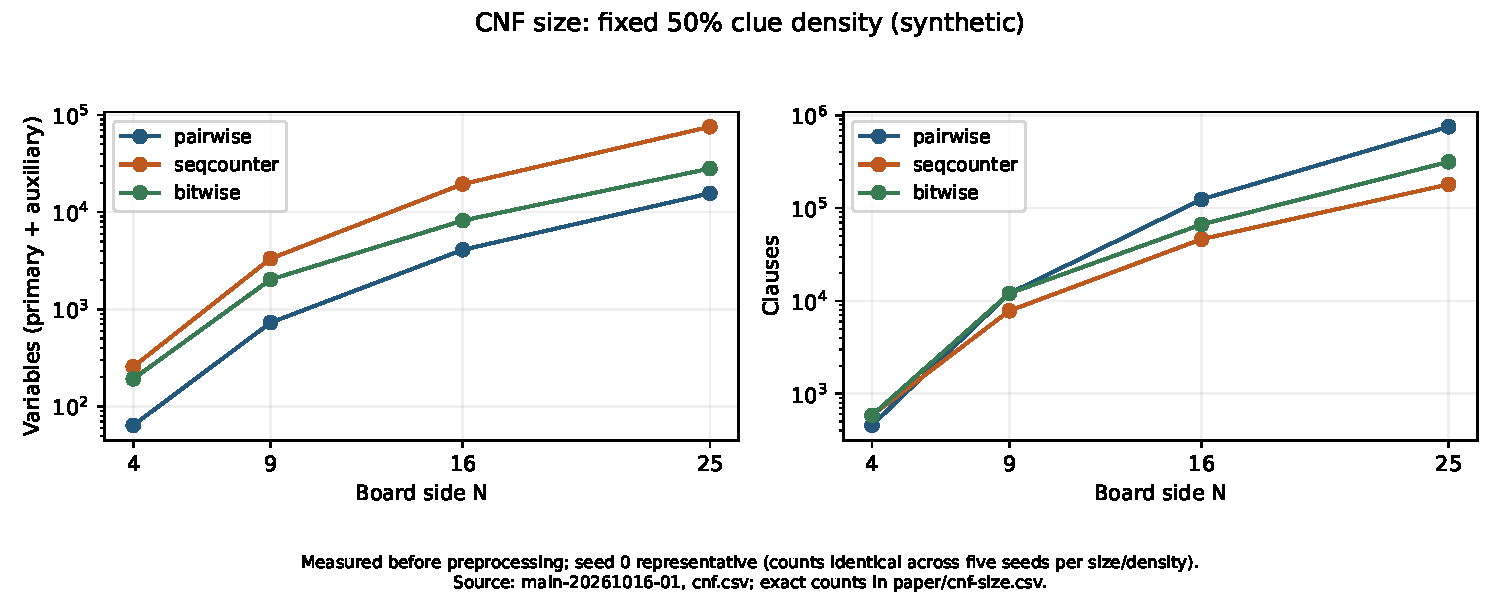
\includegraphics[width=\linewidth]{figures/figure-cnf-size.pdf}
\caption{\lang{Kích thước CNF synthetic, mật độ clue cố định 50\%; seed 0 mỗi kích thước, count trước preprocessing.}{Synthetic CNF size at fixed 50\% clue density; seed 0 at each size, before preprocessing.}}
\label{fig:cnfsize}
\end{figure}
\begin{table}[pos=H]
\centering
\small
\caption{\lang{CNF thực của synthetic-N25-p30-s0, 188 clues; trước preprocessing.}{Measured CNF for synthetic-N25-p30-s0, 188 clues; before preprocessing.}}
\label{tab:cnfactual}
\begin{tabular}{lrrrr}
\toprule
Encoding & \lang{Biến chính}{Primary} & \lang{Biến phụ}{Auxiliary} & \lang{Tổng biến}{Total variables} & Clauses\\
\midrule
pairwise & 15625 & 0 & 15625 & 752688\\
sequential & 15625 & 60000 & 75625 & 180188\\
bitwise & 15625 & 12500 & 28125 & 315188\\
\bottomrule
\end{tabular}
\end{table}


\lang{Bảng~\ref{tab:buildsolve} dùng cùng năm ID \texttt{synthetic-N25-p30-s0} đến \texttt{s4}, mỗi ID đủ ba SAT ở cả ba encoding. Build (gồm tạo/nạp solver) lớn hơn solve trong nhóm này. Sequential có median total thấp nhất, dù median solve của bitwise thấp hơn sequential. Vì vậy, chỉ xét solve hoặc số biến sẽ bỏ qua chi phí quan trọng của pipeline.}{Table~\ref{tab:buildsolve} uses the same five IDs, \texttt{synthetic-N25-p30-s0} through \texttt{s4}, each with three SAT runs for all encodings. Build, including solver creation/loading, exceeds solve time in this stratum. Sequential has the lowest median total even though bitwise has a lower median solve time. Thus solve-only timing or variable counts omit a substantial pipeline cost.}
\begin{table}[pos=H]
\centering
\small
\caption{\lang{Synthetic $25\times25$, 30\% clues: năm ID chung, giây.}{Synthetic $25\times25$, 30\% clues: five common IDs, seconds.}}
\label{tab:buildsolve}
\begin{tabular}{lrrr}
\toprule
Encoding & Median build & Median solve & Median total\\
\midrule
pairwise & 0.381882 & 0.022380 & 0.402449\\
sequential & 0.130810 & 0.024383 & 0.159527\\
bitwise & 0.193860 & 0.015416 & 0.210650\\
\bottomrule
\end{tabular}
\par\smallskip\begin{minipage}{0.97\linewidth}\footnotesize
\lang{Mỗi cột là median của median ba lượt theo đề, tổng hợp độc lập; không cộng hai median nhóm để suy median total.}{Each column is an independently aggregated median of per-instance three-run medians; the group build and solve medians do not sum to the group total median.}
\end{minipage}
\end{table}

\lang{Hình~\ref{fig:runtime} giữ riêng ba mật độ; mỗi điểm là median của năm median theo đề, mỗi median đề từ ba lần lặp. Thứ tự không cố định: ở synthetic $4\times4$/30\%, median total pairwise/sequential/bitwise lần lượt là \PairSmallTotal/\SeqSmallTotal/\BitSmallTotal{} giây. Sequential thấp nhất ở N25/30\% không đồng nghĩa thấp nhất cho mọi $n$ hoặc mọi dataset.}{Figure~\ref{fig:runtime} separates the three densities; each point is the median of five per-instance medians, each based on three repetitions. Rankings are not fixed: for synthetic $4\times4$/30\%, pairwise/sequential/bitwise median totals are \PairSmallTotal/\SeqSmallTotal/\BitSmallTotal{} seconds. Sequential's lowest total at N25/30\% does not imply the lowest time for every $n$ or dataset.}
\begin{figure}[pos=H]
\centering
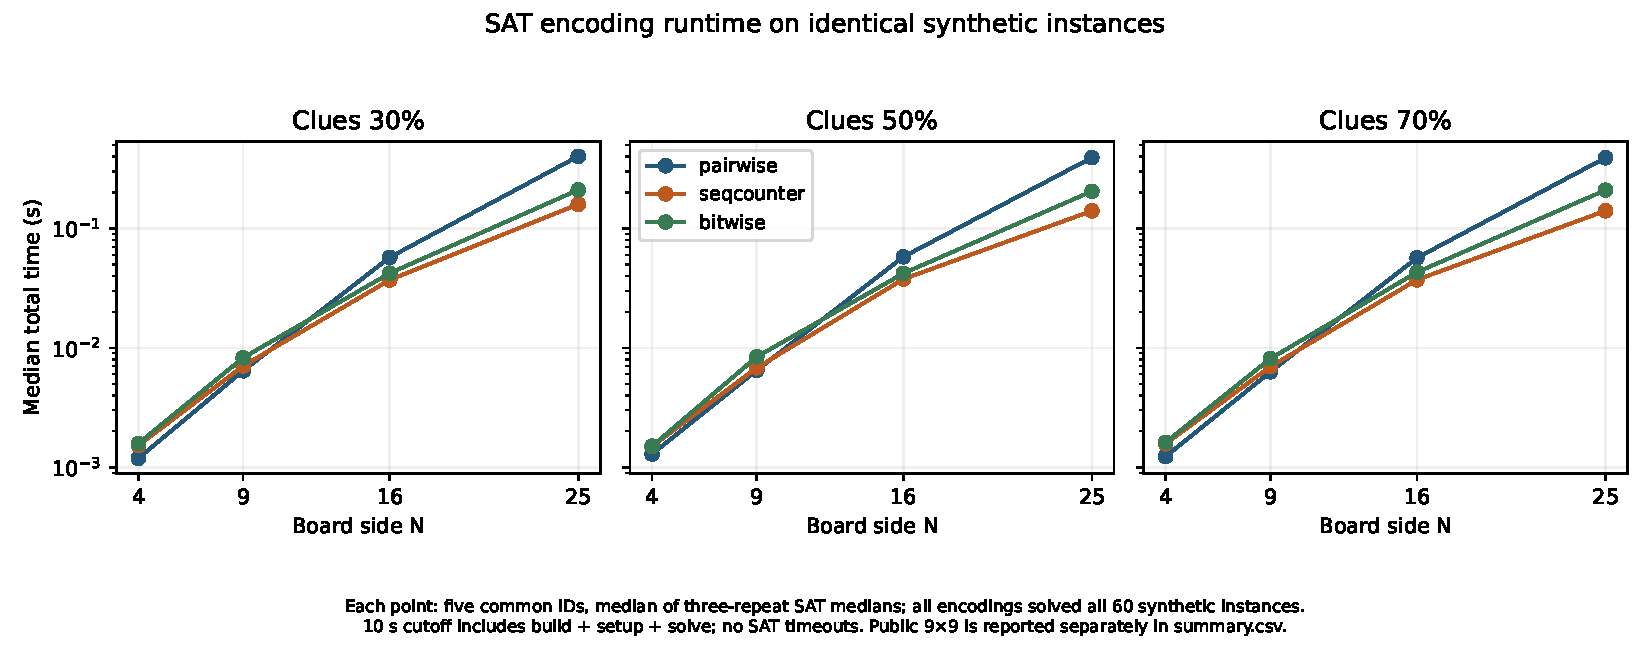
\includegraphics[width=\linewidth]{figures/figure-runtime.pdf}
\caption{\lang{Median total SAT (giây), cùng năm synthetic ID mỗi điểm; ba lần lặp/ID, cutoff 10 giây gồm build (đã gồm setup) + solve. Ba encoding không có timeout.}{SAT median total (seconds), five common synthetic IDs per point; three repetitions/ID, with a 10-second cutoff for build (including setup) + solve. No SAT encoding times out.}}
\label{fig:runtime}
\end{figure}

\subsection{\lang{Đối chứng trên đúng tập giao}{Baselines on matching instance sets}}
\lang{Các Bảng~\ref{tab:b16}--\ref{tab:public} lấy từ \texttt{paper/baseline-matched.csv}, dùng pairwise làm mốc cố định, không chọn encoding nhanh nhất riêng cho từng đối thủ. Median total chỉ lấy ID có đủ ba SAT ở cả hai bên. Trên B16, mỗi mật độ tại N25 chỉ có một ID, khác năm ID của thống kê S80 trong Bảng~\ref{tab:buildsolve}. Ví dụ \texttt{synthetic-N25-p30-s0}: CP-SAT 0.230552 giây so với pairwise 0.394866 giây; không thay giá trị pairwise này bằng \PairTotal{} giây của nhóm năm ID.}{Tables~\ref{tab:b16}--\ref{tab:public} come from \texttt{paper/baseline-matched.csv}, using pairwise as a fixed reference rather than choosing the fastest encoding separately for each opponent. Median totals include only IDs with three SAT runs in both configurations. In B16 each density at N25 has one ID, unlike the five-ID S80 statistic in Table~\ref{tab:buildsolve}. For example, on \texttt{synthetic-N25-p30-s0}, CP-SAT takes 0.230552 seconds versus pairwise's 0.394866 seconds; the latter must not be replaced by the five-ID median of \PairTotal{} seconds.}
\begin{table}[pos=H]
\centering
\small
\caption{\lang{B16 synthetic: median total trên từng ID chung, giây.}{B16 synthetic: median total on each common ID, seconds.}}
\label{tab:b16}
\begin{tabular}{rrrrrr}
\toprule
$N$ & \lang{Clues (\%)}{Clues (\%)} & $m_{CP}/m_H$ & CP-SAT & HiGHS & Pairwise\\
\midrule
4 & 30 & 1/1 & 0.004866 & 0.001704 & 0.001184\\
4 & 50 & 1/1 & 0.004223 & 0.001638 & 0.001453\\
4 & 70 & 1/1 & 0.004099 & 0.001468 & 0.001323\\
9 & 30 & 1/1 & 0.013557 & 0.012148 & 0.006350\\
9 & 50 & 1/1 & 0.006484 & 0.004400 & 0.006544\\
9 & 70 & 1/1 & 0.005491 & 0.004467 & 0.006700\\
16 & 30 & 1/1 & 0.057879 & 0.047280 & 0.057086\\
16 & 50 & 1/1 & 0.009205 & 0.021862 & 0.058682\\
16 & 70 & 1/1 & 0.007168 & 0.022792 & 0.055755\\
25 & 30 & 1/0 & 0.230552 & -- & 0.394866\\
25 & 50 & 1/1 & 0.055806 & 0.113672 & 0.382179\\
25 & 70 & 1/1 & 0.012724 & 0.066873 & 0.383525\\
\bottomrule
\end{tabular}
\par\smallskip\begin{minipage}{0.97\linewidth}\footnotesize
\lang{$m$ là số ID đủ ba SAT ở cả hai bên. Mỗi hàng chỉ có một ID, khác năm ID/hàng của S80. Dấu --: HiGHS có 3 TIMEOUT ở N25/30\%, không có median SAT.}{Here $m$ counts IDs with three SAT runs in both configurations. Each row has one ID, unlike five IDs per S80 stratum. A dash denotes three HiGHS timeouts at N25/30\%, with no SAT median.}
\end{minipage}
\end{table}

\begin{table}[pos=H]
\centering
\small
\caption{\lang{C10 synthetic: một ID chung mỗi hàng, median total (giây).}{C10 synthetic: one common ID per row, median total (seconds).}}
\label{tab:c10}
\begin{tabular}{rrrrrrr}
\toprule
$N$ & Clues (\%) & $m$ & Gurobi & CPLEX MIP & CP Optimizer & Pairwise\\
\midrule
4 & 30 & 1 & 0.002521 & 0.002137 & 0.029427 & 0.001184\\
4 & 50 & 1 & 0.002477 & 0.002280 & 0.033032 & 0.001453\\
4 & 70 & 1 & 0.002210 & 0.002362 & 0.030086 & 0.001323\\
9 & 30 & 1 & 0.010647 & 0.006728 & 0.029006 & 0.006350\\
9 & 50 & 1 & 0.007375 & 0.003787 & 0.029938 & 0.006544\\
9 & 70 & 1 & 0.007339 & 0.003884 & 0.030118 & 0.006700\\
\bottomrule
\end{tabular}
\end{table}

\begin{table}[pos=H]
\centering
\small
\caption{\lang{Bốn public $9\times9$ chung của B16/C10, median total (giây).}{Four common public $9\times9$ instances in B16/C10, median total (seconds).}}
\label{tab:public}
\begin{tabular}{llrrr}
\toprule
\lang{Backend}{Backend} & \lang{Tập}{Scope} & $m$ & \lang{Backend}{Backend} & Pairwise\\
\midrule
CP-SAT & B16 & 4 & 0.006506 & 0.006534\\
HiGHS ILP & B16 & 4 & 0.004704 & 0.006534\\
Gurobi MIP & C10 & 4 & 0.008019 & 0.006534\\
CPLEX MIP & C10 & 4 & 0.004748 & 0.006534\\
CP Optimizer & C10 & 4 & 0.030911 & 0.006534\\
\bottomrule
\end{tabular}
\par\smallskip\begin{minipage}{0.97\linewidth}\footnotesize
\lang{Cùng bốn ID L069940, L293964, L269904, L215069 (prefix public-se-hard-). Pairwise là mốc cố định; không chọn encoding nhanh nhất cho từng đối thủ.}{The same four IDs are L069940, L293964, L269904, and L215069 (prefix public-se-hard-). Pairwise is a fixed reference, not the fastest encoding selected separately for each opponent.}
\end{minipage}
\end{table}

\lang{Trên cùng bốn public, CPLEX MIP có median total \CplexPublicTotal{} giây, thấp hơn pairwise \PairPublicTotal{} giây; Gurobi \GurobiPublicTotal{} và CP Optimizer \CpoPublicTotal{} giây cao hơn pairwise. Đây là ví dụ chống nhận định SAT luôn thắng, không phải bằng chứng ILP hoặc một solver luôn tốt nhất. Các bảng không báo ratio; nếu cần ratio theo cặp phải lấy median của ratio từng ID, không chia hai median nhóm. Chênh lệch millisecond trên tập nhỏ cần được diễn giải thận trọng.}{On the same four public instances, CPLEX MIP has a median total of \CplexPublicTotal{} seconds, below pairwise's \PairPublicTotal{} seconds; Gurobi at \GurobiPublicTotal{} and CP Optimizer at \CpoPublicTotal{} seconds are higher than pairwise. This counters an assertion that SAT always wins; it does not establish that ILP or one solver is always best. Ratios are not reported in these tables; a paired ratio would require the median of per-ID ratios rather than division of group medians. Millisecond differences on a small sample require caution.}

\subsection{\lang{Timeout, PAR-2 và truy vết}{Timeouts, PAR-2, and traceability}}
\lang{Cả ba timeout là ba lần lặp HiGHS của \texttt{synthetic-N25-p30-s0}. ID này không có median SAT; tập giao runtime HiGHS với SAT/CP-SAT trên B16 còn 15 ID, còn với thương mại trên C10 vẫn 10 ID. Hai encoding SAT có 80 ID chung. Mỗi timeout nhận PAR-2 $=2\times10=20$ giây, tổng ba penalty là 60 giây; mean PAR-2 của đúng nhóm HiGHS N25/30\% là 20 giây. Không coi timing thiếu là 0: r3 thiếu cả build/solve/total vẫn để thiếu, r1/r2 có observed total khoảng cutoff nhưng vẫn TIMEOUT. Runtime của phần giải được luôn phải đọc cùng count trong Bảng~\ref{tab:coverage}.}{All three timeouts are the three HiGHS repetitions of \texttt{synthetic-N25-p30-s0}. This ID has no SAT median; the runtime intersection between HiGHS and SAT/CP-SAT on B16 contains 15 IDs, while its intersection with commercial engines on C10 still contains 10. Two SAT encodings share 80 IDs. Each timeout receives PAR-2 $=2\times10=20$ seconds, for a total timeout penalty of 60 seconds; mean PAR-2 for the HiGHS N25/30\% stratum is 20 seconds. Missing timings are not zero: r3 lacks build/solve/total and remains missing, while r1/r2 have observed totals near the cutoff but remain TIMEOUT. Successful-only runtime statistics must be read with the counts in Table~\ref{tab:coverage}.}
\lang{Các bảng/hình lấy từ analysis final đã khóa; \texttt{summary.csv}, \texttt{instances.csv}, \texttt{matched-pairs.csv} và \texttt{cnf.csv} giữ thống kê chi tiết. \texttt{paper/raw-row-index.csv} nối job ID tới dòng CSV gốc; audit giữ config, phiên bản và hash. Không gộp pilot, không chạy lại benchmark để chọn kết quả thuận lợi.}{Tables and figures use the locked final analysis; \texttt{summary.csv}, \texttt{instances.csv}, \texttt{matched-pairs.csv}, and \texttt{cnf.csv} retain detailed statistics. \texttt{paper/raw-row-index.csv} maps job IDs to original CSV rows; the audit retains configuration, versions, and hashes. Pilot data are not merged, and the benchmark is not rerun to select favorable results.}
